\documentclass[12pt, titlepage]{article}

\usepackage{fullpage}
\usepackage[round]{natbib}
\usepackage{multirow}
\usepackage{booktabs}
\usepackage{tabularx}
\usepackage{graphicx}
\usepackage{float}
\usepackage{indentfirst}
\usepackage{hyperref}
\hypersetup{
    colorlinks,
    citecolor=black,
    filecolor=black,
    linkcolor=red,
    urlcolor=blue
}
\usepackage[round]{natbib}

\newcounter{acnum}
\newcommand{\actheacnum}{AC\theacnum}
\newcommand{\acref}[1]{AC\ref{#1}}

\newcounter{ucnum}
\newcommand{\uctheucnum}{UC\theucnum}
\newcommand{\uref}[1]{UC\ref{#1}}

\newcounter{mnum}
\newcommand{\mthemnum}{M\themnum}
\newcommand{\mref}[1]{M\ref{#1}}

\title{SFWRENG 3XA3: Module Guide\\Rummy For Dummies}

\author{Lab 2 Group 7, Rummy For Dummies
		\\ Joy Xiao, xiaoz18
		\\ Benson Hall, hallb8
		\\ Smita Singh, sings59
}

\date{March 18, 2021}

\begin{document}

\maketitle

\pagenumbering{roman}
\tableofcontents
\listoftables
\listoffigures

\begin{table}[bp]
    \caption{\bf Revision History}
    \begin{tabularx}{\textwidth}{p{3cm}p{2cm}X}
        \toprule {\bf Date} & {\bf Version} & {\bf Notes}\\
        \midrule
        March 16, 2021 & 1.0 & Started on the MG\\
        March 18, 2021 & 1.1 & Finished the MG\\
        \bottomrule
    \end{tabularx}
\end{table}

\newpage

\pagenumbering{arabic}

\section{Introduction}
\subsection{Overview}
Rummy For Dummies is a Java re-implementation of the card game Gin Rummy. The intent is to recreate a single-player card game normally played with several people. This is to provide users the experience of playing a multi-player card game. 

Rummy For Dummies will be an improved version of the original open-source project played on the command line. This is done through being more user-friendly compared to the open-source implementation and more accessible to the general public, even if they do not have a technical background. This will be achieved in both the documentation and the game itself.

\subsection{Context}
Decomposing a system into modules is a commonly accepted approach to developing software. A module is a work assignment for a programmer or programming team ~\citep{ParnasEtAl1984}.
We advocate a decomposition based on the principle of information hiding ~\citep{Parnas1972a}.
This principle supports design for change, because the ``secrets'' that each module hides represent likely future changes.  Design for change is valuable in SC, where modifications are frequent, especially during initial development as the solution space is explored.  

Our design follows the rules laid out by \citet{ParnasEtAl1984}, as follows:
\begin{itemize}
    \item System details that are likely to change independently should be the secrets of separate modules.
    \item Each data structure is used in only one module.
    \item Any other program that requires information stored in a module's data
      structures must obtain it by calling access programs belonging to that module.
\end{itemize}

After completing the first stage of the design, the Software Requirements Specification (SRS), the Module Guide (MG) is developed ~\citep{ParnasEtAl1984}. The MG specifies the modular structure of the system and is intended to allow both designers and maintainers to easily identify the parts of the software. The potential readers of this document are as follows:

\begin{itemize}
    \item New project members: This document can be a guide for a new project member
      to easily understand the overall structure and quickly find the
      relevant modules they are searching for.
    \item Maintainers: The hierarchical structure of the module guide improves the
      maintainers' understanding when they need to make changes to the system. It is
      important for a maintainer to update the relevant sections of the document
      after changes have been made.
    \item Designers: Once the module guide has been written, it can be used to
      check for consistency, feasibility and flexibility. Designers can verify the
      system in various ways, such as consistency among modules, feasibility of the
      decomposition, and flexibility of the design.
\end{itemize}

The rest of the document is organized as follows. Section
\ref{SecChange} lists the anticipated and unlikely changes of the software
requirements. Section \ref{SecMH} summarizes the module decomposition that
was constructed according to the likely changes. Section \ref{SecConnection}
specifies the connections between the software requirements and the
modules. Section \ref{SecMD} gives a detailed description of the
modules. Section \ref{SecTM} includes two traceability matrices. One checks
the completeness of the design against the requirements provided in the SRS. The
other shows the relation between anticipated changes and the modules. Section
\ref{SecUse} describes the use relation between modules.

\section{Anticipated and Unlikely Changes} \label{SecChange}

This section lists possible changes to the system. According to the likeliness
of the change, the possible changes are classified into two
categories. Anticipated changes are listed in Section \ref{SecAchange}, and
unlikely changes are listed in Section \ref{SecUchange}.

\subsection{Anticipated Changes} \label{SecAchange}

Anticipated changes are the sources of the information that is to be hidden inside the modules. Ideally, changing one of the anticipated changes will only require changing the one module that hides the associated decision. The approach adapted here is called design for change.

\begin{description}
    \item[\refstepcounter{acnum} \actheacnum \label{acHardware}:] The specific
      hardware on which the software is running.
    \item[\refstepcounter{acnum} \actheacnum \label{acH}:] The presentation of the player's hand on the console.
    \item[\refstepcounter{acnum} \actheacnum \label{acDP}:] The presentation of the discard pile on the console.
    \item[\refstepcounter{acnum} \actheacnum \label{acExc}:] The addition of exception handling to all the classes.
\end{description}

\subsection{Unlikely Changes} \label{SecUchange}

The module design should be as general as possible. However, a general system is
more complex. Sometimes this complexity is not necessary. Fixing some design
decisions at the system architecture stage can simplify the software design. If
these decision should later need to be changed, then many parts of the design
will potentially need to be modified. Hence, it is not intended that these
decisions will be changed.

\begin{description}
    \item[\refstepcounter{ucnum} \uctheucnum \label{ucCO}:] The computer opponent playing algorithm. 
    \item[\refstepcounter{ucnum} \uctheucnum \label{ucM}:] The meld algorithm to find melds in a hand. 
    \item[\refstepcounter{ucnum} \uctheucnum \label{ucSP}:] The data structure for the stock pile. 
    \item[\refstepcounter{ucnum} \uctheucnum \label{ucDP}:] The data structure for the discard pile. 
    \item[\refstepcounter{ucnum} \uctheucnum \label{ucH}:] The data structure for the hand. 
    \item[\refstepcounter{ucnum} \uctheucnum \label{ucC}:] The data structure for the card. 
    \item[\refstepcounter{ucnum} \uctheucnum \label{ucInput}:] There will always be a source of input data external to the software.
    \item[\refstepcounter{ucnum} \uctheucnum \label{ucP}:] The data structure for the player.
    \item[\refstepcounter{ucnum} \uctheucnum \label{ucG}:] The algorithms for the game's basic functions.
\end{description}

\section{Module Hierarchy} \label{SecMH}

This section provides an overview of the module design. Modules are summarized
in a hierarchy decomposed by secrets in Table \ref{TblMH}. The modules listed
below, which are leaves in the hierarchy tree, are the modules that will
actually be implemented.

\begin{description}
\item [\refstepcounter{mnum} \mthemnum \label{mHH}:] Hardware-Hiding Module

\item [\refstepcounter{mnum}
 \mthemnum \label{mGO}:] Game Operations Module

\item [\refstepcounter{mnum} \mthemnum \label{mI}:] Input Module

\item [\refstepcounter{mnum} \mthemnum \label{mC}:] Computer Module

\item [\refstepcounter{mnum} \mthemnum \label{mSP}:] Stock Pile Data Structure Module

\item [\refstepcounter{mnum} \mthemnum \label{mDP}:] Discard Pile Data Structure Module

\item [\refstepcounter{mnum} \mthemnum \label{mCard}:] Card Data Structure Module

\item [\refstepcounter{mnum} \mthemnum \label{mH}:] Hand Data Structure Module

\item [\refstepcounter{mnum}
\mthemnum \label{mM}:] Melds Module

\item [\refstepcounter{mnum}
\mthemnum \label{mP}:] Player Data Structure Module
\end{description}


\begin{table}[H]
    \centering
    \begin{tabular}{p{0.3\textwidth} p{0.6\textwidth}}
        \toprule
        \textbf{Level 1} & \textbf{Level 2}\\
        \midrule
        
        {Hardware-Hiding Module} & ~ \\
        \midrule
        
        \multirow{3}{0.3\textwidth}{Behaviour-Hiding Module}\\
        & Game Operations Module\\
        & Input Module\\
        & Melds Module\\
        \midrule
        
        \multirow{3}{0.3\textwidth}{Software Decision Module}\\
        & Computer Module\\
        & Stock Pile Data Structure Module\\
        & Discard Pile Data Structure Module\\
        & Card Data Structure Module\\
        & Hand Data Structure Module\\
        & Player Data Structure Module\\
        \bottomrule
        
    \end{tabular}
    \caption{Module Hierarchy}
    \label{TblMH}
\end{table}

\section{Connection Between Requirements and Design} \label{SecConnection}

The design of the system is intended to satisfy the requirements developed in
the SRS. In this stage, the system is decomposed into modules. The connection
between requirements and modules is listed in Table \ref{TblRT}.

\section{Module Decomposition} \label{SecMD}

Modules are decomposed according to the principle of ``information hiding''
proposed by \citet{ParnasEtAl1984}. The \emph{Secrets} field in a module
decomposition is a brief statement of the design decision hidden by the
module. The \emph{Services} field specifies \emph{what} the module will do
without documenting \emph{how} to do it. For each module, a suggestion for the
implementing software is given under the \emph{Implemented By} title. If the
entry is \emph{OS}, this means that the module is provided by the operating
system or by standard programming language libraries.  Also indicate if the
module will be implemented specifically for the software.

Only the leaf modules in the
hierarchy have to be implemented. If a dash (\emph{--}) is shown, this means
that the module is not a leaf and will not have to be implemented. Whether or
not this module is implemented depends on the programming language
selected.

\subsection{Hardware Hiding Modules (\mref{mHH})}

\begin{description}
    \item[Secrets:]The data structure and algorithm used to implement the virtual
      hardware.
    \item[Services:]Serves as a virtual hardware used by the rest of the system. This module provides the interface between the hardware and the software. So, the system can use it to display outputs or to accept inputs.
    \item[Implemented By:] OS, Java
\end{description}

\subsection{Behaviour-Hiding Module}

\subsubsection{Game Operations Module (\mref{mGO})}
\begin{description}
    \item[Secrets:]The algorithms representing the game's functions
    \item[Services:]Uses the algorithms to perform the game's basic functions 
    \item[Implemented By:]GameOps.java
\end{description}

\subsubsection{Input Module (\mref{mI})}

\begin{description}
    \item[Secrets:]The methods for taking user data and formatting it to be usable for the data structures and algorithms of the game.
    \item[Services:]Accepts and converts input data into data that will be used by the game operations module.
    \item[Implemented By:]UserInputOps.java
\end{description}

\subsubsection{Melds Module (\mref{mM})}
\begin{description}
    \item[Secrets:]The algorithm used to determine optimal melds
    \item[Services:]Determines optimal melds from a hand of cards, and returns a 2D ArrayList of sequence and group melds. 
    \item[Implemented By:]Meld.java, SortByRank.java, SortBySR.java
\end{description}
\subsection{Software Decision Module}

\subsubsection{Computer Module (\mref{mC})}
\begin{description}
    \item[Secrets:]The algorithm of the computer module.
    \item[Services:]Performs the computer opponent move with a specific algorithm used.
    \item[Implemented By:] Computer.java
\end{description}

\subsubsection{Stock Pile Data Structure Module (\mref{mSP})}
\begin{description}
    \item[Secrets:]The data structure of the stock pile for the game.
    \item[Services:]Stores the information about the stock pile such as the order of cards, as well as functionalities such as adding and removing cards. 
    \item[Implemented By:]StockPile.java
\end{description}

\subsubsection{Discard Pile Data Structure Module (\mref{mDP})}
\begin{description}
    \item[Secrets:]The data structure of the discard pile for the game.
    \item[Services:]Stores the information about the discard pile such as the order of cards, as well as functionalities such as adding and removing cards. It also stores the information for displaying the discard pile on the console. 
    \item[Implemented By:] DiscardPile.java
\end{description}

\subsubsection{Card Data Structure (\mref{mCard})}
\begin{description}
    \item[Secrets:]The data structure for the cards in the game
    \item[Services:]Stores information of card objects as well as provides other functionalities
    \item [Implemented by:]Card.java
\end{description}

\subsubsection{Hand Data Structure Module (\mref{mH})}
\begin{description}
    \item[Secrets:] The data structure of a hand in the game.
    \item[Services:] Stores the information about a hand of cards as well as functionalities such as removing a card from the hand and adding a card to the hand.
    \item[Implemented By:] Hand.java
\end{description}


\subsubsection{Player Data Structure Module (\mref{mP})}
\begin{description}
    \item[Secrets:]The data structure of a player in the game
    \item[Services:]Stores information about a player, as well as interfacing methods for performing operations on its internal state objects
    \item[Implemented By:]Player.java
\end{description}

\section{Traceability Matrix} \label{SecTM}

This section shows two traceability matrices: between the modules and the
requirements and between the modules and the anticipated changes.

% the table should use mref, the requirements should be named, use something
% like fref
\begin{table}[H]
    \centering
    \begin{tabular}{p{0.2\textwidth} p{0.6\textwidth}}
        \toprule
        \textbf{Req.} & \textbf{Modules}\\
        \midrule
        FR1 & \mref{mGO}, \mref{mI} \\
        FR2 & \mref{mGO}, \mref{mCard}, \mref{mDP}, \mref{mH}, \mref{mP} \\
        FR3 & \mref{mGO}, \mref{mI} \\
        FR4 & \mref{mGO}, \mref{mSP}, \mref{mCard}, \mref{mH}, \mref{mP} \\
        FR5 & \mref{mGO} \\
        FR6 & \mref{mI} \\
        FR7 & \mref{mGO}, \mref{mDP}, \mref{mCard}, \mref{mH}, \mref{mP} \\
        FR8 & \mref{mGO} \\
        FR9 & \mref{mI} \\
        FR10 & \mref{mGO}, \mref{mCard}, \mref{mH}, \mref{mM}, \mref{mP} \\
        FR11 & \mref{mGO}, \mref{mP} \\
        FR12 & \mref{mGO}, \mref{mI}, \mref{mCard}, \mref{mH}, \mref{mP} \\
        FR13 & \mref{mGO}, \mref{mDP}, \mref{mCard}, \mref{mH}, \mref{mP} \\
        FR14 & \mref{mGO}, \mref{mDP}, \mref{mCard} \\
        FR15 & \mref{mGO}, \mref{mP}, \mref{mC}, \mref{mCard}, \mref{mSP}, \mref{mDP} \\
        FR16 & \mref{mGO}, \mref{mP} \\
        FR17 & \mref{mGO} \\
        FR18 & \mref{mGO}, \mref{mP} \\
        FR19 & \mref{mGO}, \mref{mP} \\
        FR20 & \mref{mGO}, \mref{mI} \\
        FR21 & \mref{mGO}, \mref{mI} \\
        LF1 & \mref{mGO} \\
        UH1 & \mref{mGO} \\
        UH2 & \mref{mGO} \\
        P1 & \mref{mGO} \\
        P2 & \mref{mGO} \\
        OE1 & \mref{mGO} \\
        MS1 & \mref{mGO}, \mref{mI}, \mref{mC}, \mref{mSP}, \mref{mDP},\mref{mCard}, \mref{mH}, \mref{mM}, \mref{mP} \\
        MS2 & \mref{mGO}, \mref{mI}, \mref{mC}, \mref{mSP}, \mref{mDP}, \mref{mCard}, \mref{mH}, \mref{mM}, \mref{mP} \\
        C1 & \mref{mGO} \\
        C2 & \mref{mGO} \\
        L1 & \mref{mGO}, \mref{mI}, \mref{mC}, \mref{mSP}, \mref{mDP}, \mref{mCard}, \mref{mH}, \mref{mM}, \mref{mP} \\
        \bottomrule
    \end{tabular}
    \caption{Trace Between Requirements and Modules}
    \label{TblRT}
\end{table}

\begin{table}[H]
\centering
\begin{tabular}{p{0.2\textwidth} p{0.6\textwidth}}
\toprule
\textbf{AC} & \textbf{Modules}\\
\midrule
\acref{acHardware} & \mref{mHH}\\
\acref{acH} & \mref{mH}\\
\acref{acDP} & \mref{mDP}\\
\acref{acExc} & \mref{mGO}, \mref{mI}, \mref{mC}, \mref{mSP}, \mref{mDP}, \mref{mCard}, \mref{mH}, \mref{mM}, \mref{mP}\\
\bottomrule
\end{tabular}
\caption{Trace Between Anticipated Changes and Modules}
\label{TblACT}
\end{table}

\section{Use Hierarchy Between Modules} \label{SecUse}

In this section, the uses hierarchy between modules is
provided. \citet{Parnas1978} said of two programs A and B that A {\em uses} B if
correct execution of B may be necessary for A to complete the task described in
its specification. That is, A {\em uses} B if there exist situations in which
the correct functioning of A depends upon the availability of a correct
implementation of B. Figure \ref{FigUH} illustrates the use relation between
the modules. It can be seen that the graph is a directed acyclic graph
(DAG). Each level of the hierarchy offers a testable and usable subset of the
system, and modules in the higher level of the hierarchy are essentially simpler
because they use modules from the lower levels.



\begin{figure}[H]
    \centering
    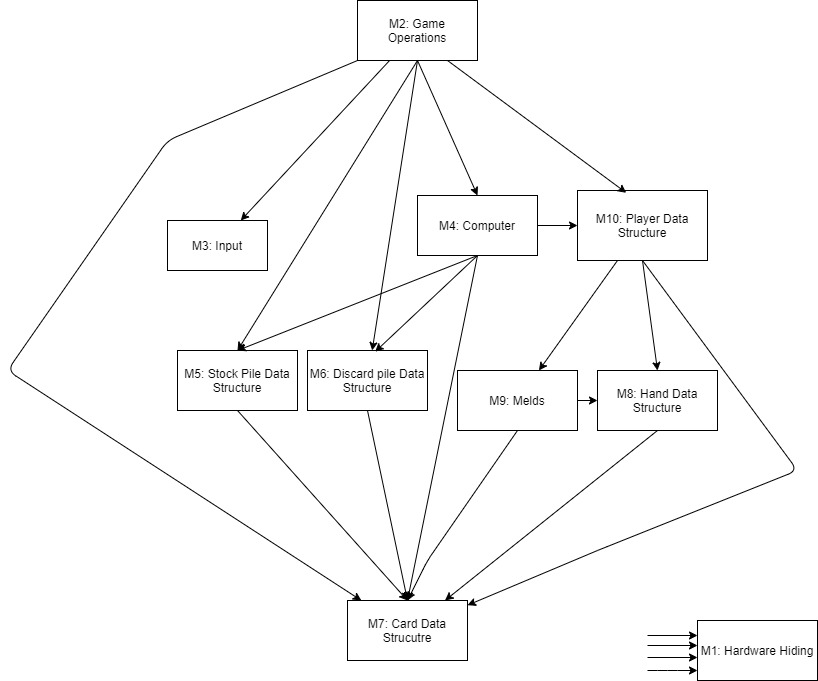
\includegraphics[width=\textwidth]{user_hierarchy.jpg}
    \caption{Use hierarchy among modules}
    \label{FigUH}
\end{figure}

\section{Project Schedule}
The Gantt Chart for the project schedule is located under the \textit{ProjectSchedule} directory, named \textbf{3XA3-project.gan}.
%\section*{References}

\bibliographystyle {plainnat}
\bibliography {MG}

\end{document}